%%%%%%%%%%%%%%%%%%%%%%%%%%%%%%%%%%%%%%%%%
% Simple Sectioned Essay Template
% LaTeX Template
%
% This template has been downloaded from:
% http://www.latextemplates.com
%
% Note:
% The \lipsum[#] commands throughout this template generate dummy text
% to fill the template out. These commands should all be removed when 
% writing essay content.
%
%%%%%%%%%%%%%%%%%%%%%%%%%%%%%%%%%%%%%%%%%

%----------------------------------------------------------------------------------------
%	PACKAGES AND OTHER DOCUMENT CONFIGURATIONS
%----------------------------------------------------------------------------------------

\documentclass[12pt]{article} % Default font size is 12pt

\usepackage[utf8]{inputenc}

\usepackage[a4paper]{geometry} % Required to change the page size to A4
% Set the page size to be A4 as opposed to the default US Letter

\usepackage{float} % Allows putting an [H] in \begin{figure} to specify the exact location of the figure
\usepackage{wrapfig} % Allows in-line images such as the example fish picture

\usepackage{lipsum} % Used for inserting dummy 'Lorem ipsum' text into the template

\usepackage{amsmath}
\usepackage{amsthm}
\usepackage{amssymb}

\usepackage{epigraph}

\usepackage[numbers, sort]{natbib}
\bibliographystyle{plainnat}

\usepackage[nottoc]{tocbibind}

\usepackage{makeidx}
\makeindex

\linespread{1.2} % Line spacing

%\setlength\parindent{0pt} % Uncomment to remove all indentation from paragraphs

\usepackage{graphicx} % Required for including pictures
\graphicspath{{../figures/}} % Specifies the directory where pictures are stored

\usepackage{epstopdf}

\usepackage{hyperref}
\hypersetup{
    colorlinks,
    citecolor=black,
    filecolor=black,
    linkcolor=black,
    urlcolor=black
}

\usepackage{microtype}
\usepackage{siunitx}
\usepackage{cleveref}
\usepackage{booktabs}

\begin{document}

%----------------------------------------------------------------------------------------
%	TITLE PAGE
%----------------------------------------------------------------------------------------

\begin{titlepage}

\newcommand{\HRule}{\rule{\linewidth}{0.5mm}} % Defines a new command for the horizontal lines, change thickness here

\center % Center everything on the page

\textsc{\Large The University of New South Wales}\\[0.2cm]
\textsc{\large School of Computer Science and Engineering}\\[1.5cm] % Name of your university/college

\textsc{\large Thesis Report - Part A}\\[0.5cm] % Major heading such as course name
\textsc{BSc Computer Science (Honours)}\\[0.5cm] % Minor heading such as course title

\HRule \\[0.4cm]
{ \LARGE \bfseries The Chromatic Derivatives and its Applications }\\[0.4cm] % Title of your document
\HRule \\[1.5cm]

\begin{minipage}[t]{0.4\textwidth}
\begin{flushleft} \large
\emph{Author:}\\
Louis \textsc{Tiao} % Your name
\end{flushleft}
\end{minipage}
~
\begin{minipage}[t]{0.5\textwidth}
\begin{flushright} \large
\emph{Supervisor:} \\
Dr. Aleksandar \textsc{Ignjatovic} % Supervisor's Name
\\[0.5cm]
\emph{Assessor:} \\
Dr. Alan \textsc{Blair} % Assessor's Name
\end{flushright}
\end{minipage}\\[4cm]

{\large \today}\\[3cm] % Date, change the \today to a set date if you want to be precise

%\includegraphics{Logo}\\[1cm] % Include a department/university logo - this will require the graphicx package

\vfill % Fill the rest of the page with whitespace

\end{titlepage}

%----------------------------------------------------------------------------------------
%	TABLE OF CONTENTS
%----------------------------------------------------------------------------------------

\tableofcontents % Include a table of contents

\newpage % Begins the essay on a new page instead of on the same page as the table of contents 

%----------------------------------------------------------------------------------------
%	INTRODUCTION
%----------------------------------------------------------------------------------------

\section{Introduction} % Major section

In \citep{Ignjatovic2009}
\the \columnwidth


\subsection{Image processing applications}

\subsubsection{Padding for neighborhood operations}

A linear filter is a type of \emph{neighborhood operator} that uses a weighted 
combination of the pixel values in the vicinity of a given pixel to determine 
its final output value~\cite[p.~111]{Szeliski2011}.

Denote $f(i, j)$ the pixel value and let $h(k, l)$ be the \emph{convolution 
matrix} or \emph{kernel}. The \emph{convolution} between $f$ and $h$ is given by
\begin{align} \label{eq:linear_filter_convolution}
	g(i, j) = [f \ast h](i, j) 	&= \sum_k \sum_l f(i-k, j-l) \cdot h(k, l) \\
								&= \sum_k \sum_l f(k, l) \cdot h(i-k, j-l)  \nonumber
\end{align}

The linear filter can be used to create a wide range of effects, such as adding 
soft blurs, sharpening details, accentuating edges, etc.

One obvious problem that arises is that at the border of the image, the 
convolution operation requires pixel values that are outside the boundaries
of the image.

Let $\tilde{f}(i, j)$ be the padded pixel values. We can define it as a function 
of the original pixel values $f(k, l)$ and the dimension (height, width) of the 
image $(M, N)$.

\begin{align*}
  \tilde{f}(i, j) &= f(k, l), \\
  k               &= \max(0, \min(M-1, i)), \\
  l               &= \max(0, \min(N-1, j)).
\end{align*}

We would like to approximate $\tilde{f}(i, j)$ \dots

\citet[see][p.~114-115]{Szeliski2011} provides 

\subsubsection{Digital image inpainting}

\newpage

\section{Background}

\subsection{Preliminaries}

\epigraph{In mathematics you don't understand things. You just get used to them.}{John von Neumann}

\subsubsection{Taylor series}

\subsubsection{Orthogonal systems}
 
\subsubsection{Fourier series}

\subsubsection{Legendre Polynomials}

The \emph{Legendre functions} are solutions to the \emph{Legendre differential 
equation}, which is the second-order ordinary differential equation

\begin{equation} \label{eq:legendre_de}
\frac{d}{dx}\left[(1-x^2)\frac{d}{dx}P_n(x)\right]+n(n+1)P_n(x)=0
\end{equation}

The \emph{Legendre polynomials} are also known as \emph{Legendre functions of the 
first kind}, and are most conveniently defined recursively as follows:

\begin{align*}
P_0(x) &= 1, P_1(x) = x \\
P_{n+1}(x) &= \frac{2n+1}{n+1}xP_n(x) - \frac{n}{n+1}P_{n-1}(x)
\end{align*}

\begin{figure}[H] % Example image
\center{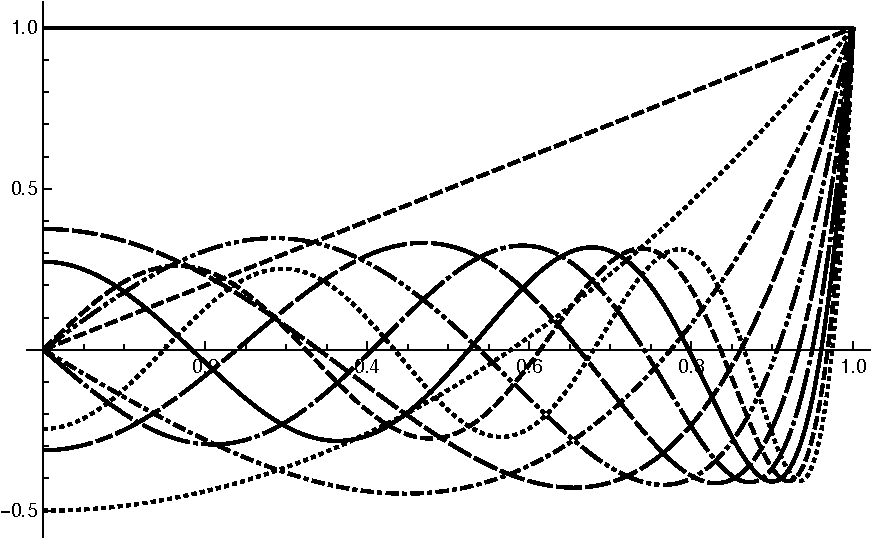
\includegraphics{legendre_bw.pdf}}
\caption{First 10 Legendre polynomials.}
\label{fig:legendre}
\end{figure}

Orthogonal and complete over $[-1, 1]$
\begin{equation*}
\int_{-1}^{1} P_n(x)P_m(x) dx = \frac{2}{2n+1} \delta_{mn}
\end{equation*}
where $\delta_{mn}$ is the Kronecker delta.

\subsection{Digital signal processing}



\subsection{Subsubsection 1} % Sub-sub-section

\lipsum[3] % Dummy text

\begin{figure}[H] % Example image
\center{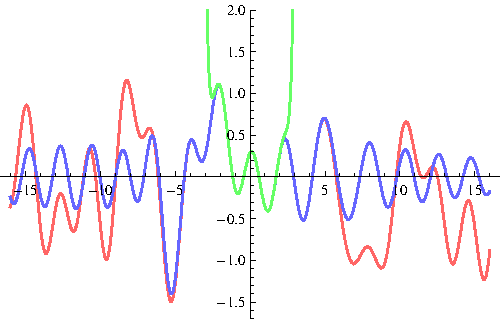
\includegraphics[width=0.5\linewidth]{approx}}
\caption{Example image.}
\label{fig:speciation}
\end{figure}

%------------------------------------------------

\subsubsection{Subsubsection 2} % Sub-sub-section

\lipsum[4] % Dummy text

%----------------------------------------------------------------------------------------
%	MAJOR SECTION 1
%----------------------------------------------------------------------------------------

\section{Proposal} % Major section

\lipsum[5] % Dummy text

%------------------------------------------------

\subsection{Subsection 1} % Sub-section

\subsubsection{Subsubsection 1} % Sub-sub-section

\lipsum[6] % Dummy text

%------------------------------------------------

\subsubsection{Subsubsection 2} % Sub-sub-section

\lipsum[6] % Dummy text
\begin{wrapfigure}{l}{0.4\textwidth} % Inline image example
  \begin{center}
    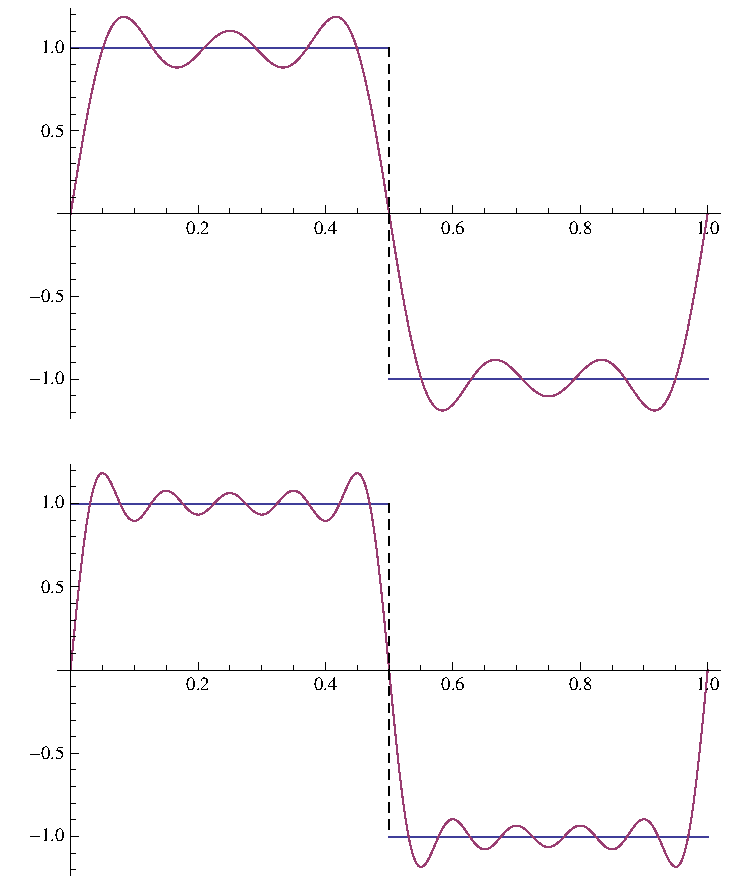
\includegraphics[width=0.38\textwidth]{fourier}
  \end{center}
  \caption{Fish}
\end{wrapfigure}
\lipsum[7-8] % Dummy text

%------------------------------------------------

\subsubsection{Subsubsection 3} % Sub-sub-section

\begin{description} % Numbered list example

\item[First] \hfill \\
\lipsum[9] % Dummy text

\item[Second] \hfill \\
\lipsum[10] % Dummy text

\item[Third] \hfill \\
\lipsum[11] % Dummy text

\end{description} 

%----------------------------------------------------------------------------------------
%	MAJOR SECTION X - TEMPLATE - UNCOMMENT AND FILL IN
%----------------------------------------------------------------------------------------

%\section{Content Section}

%\subsection{Subsection 1} % Sub-section

% Content

%------------------------------------------------

%\subsection{Subsection 2} % Sub-section

% Content

%----------------------------------------------------------------------------------------
%	CONCLUSION
%----------------------------------------------------------------------------------------

\section{Conclusion} % Major section

\lipsum[12-13]

%----------------------------------------------------------------------------------------
%	BIBLIOGRAPHY
%----------------------------------------------------------------------------------------

\bibliography{../bibliography}

%----------------------------------------------------------------------------------------
%	APPENDIX
%----------------------------------------------------------------------------------------

\appendix

\section{Code}

%----------------------------------------------------------------------------------------
%	INDEX
%----------------------------------------------------------------------------------------

\printindex

%----------------------------------------------------------------------------------------

\end{document}